\documentclass[11pt,a4paper]{scrartcl}

\usepackage{fullpage}

%\usepackage[ngerman]{babel}
\usepackage[utf8]{inputenc}
\usepackage{graphicx}

\usepackage{amsmath}
\usepackage{amsthm}
\usepackage{mathtools}

\usepackage{listings}
\usepackage{xcolor}

%%%%% COMMANDS

\newcommand{\FT}{\mathcal{F}}
\newcommand{\T}{\mathrm{T}}
\newcommand{\IFT}{\mathcal{F}^{-1}}
\newcommand{\conv}{\ast}
\newcommand{\defined}{\coloneqq}

\newtheorem*{theorem}{Theorem}



\begin{document}

\lstdefinestyle{customc}{
    belowcaptionskip=1\baselineskip,
    breaklines=true,
    xleftmargin=\parindent,
    language=Python,
    showstringspaces=false,
    basicstyle=\footnotesize\ttfamily,
    keywordstyle=\bfseries\color{green!40!black},
    commentstyle=\itshape\color{purple!40!black},
    identifierstyle=\color{blue},
    stringstyle=\color{orange}
}
\lstset{
    style=customc
} 

\title{Image Analysis Excercise Sheet 7}
\author{Markus Doering, 3153320}
\maketitle

\section{Natural Image Statistics}
All python code for this excercise is found in file \verb$ia_07_01.py$ and in the appendix. 
\begin{figure}[hb]
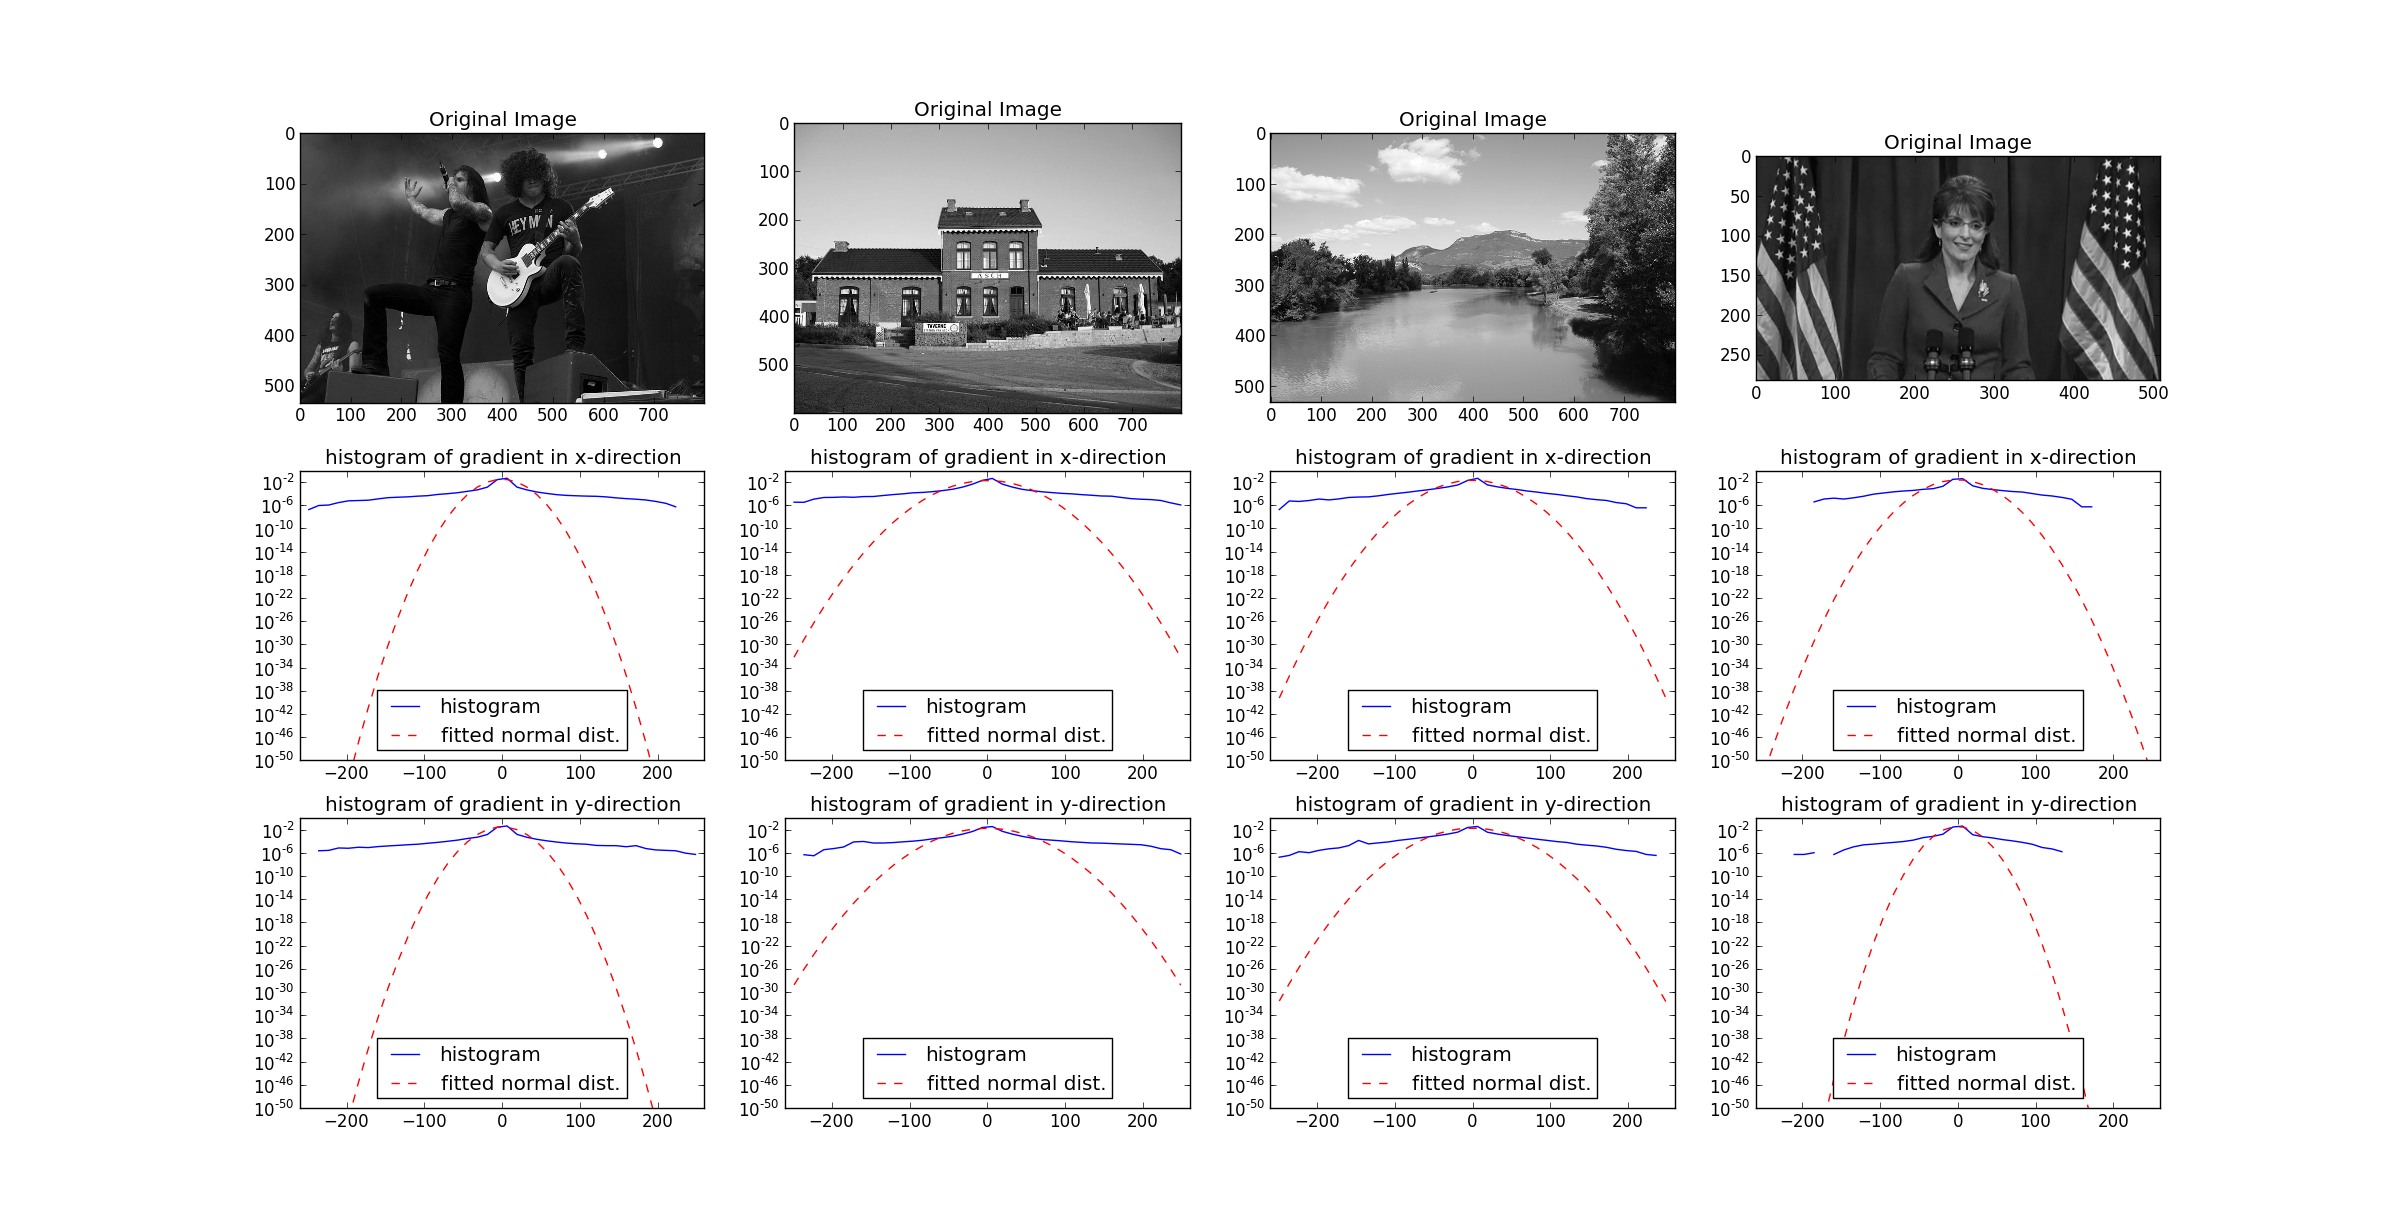
\includegraphics[width=.99\linewidth]{histograms.png}
\caption{BLALABERBLUB}
\end{figure}

\section{Factor Graphs}
TODO

\section{Integer Linear Programming}
All python code for this excercise is found in file \verb$ia_07_03.py$ and in the appendix. 
\begin{figure}[hb]
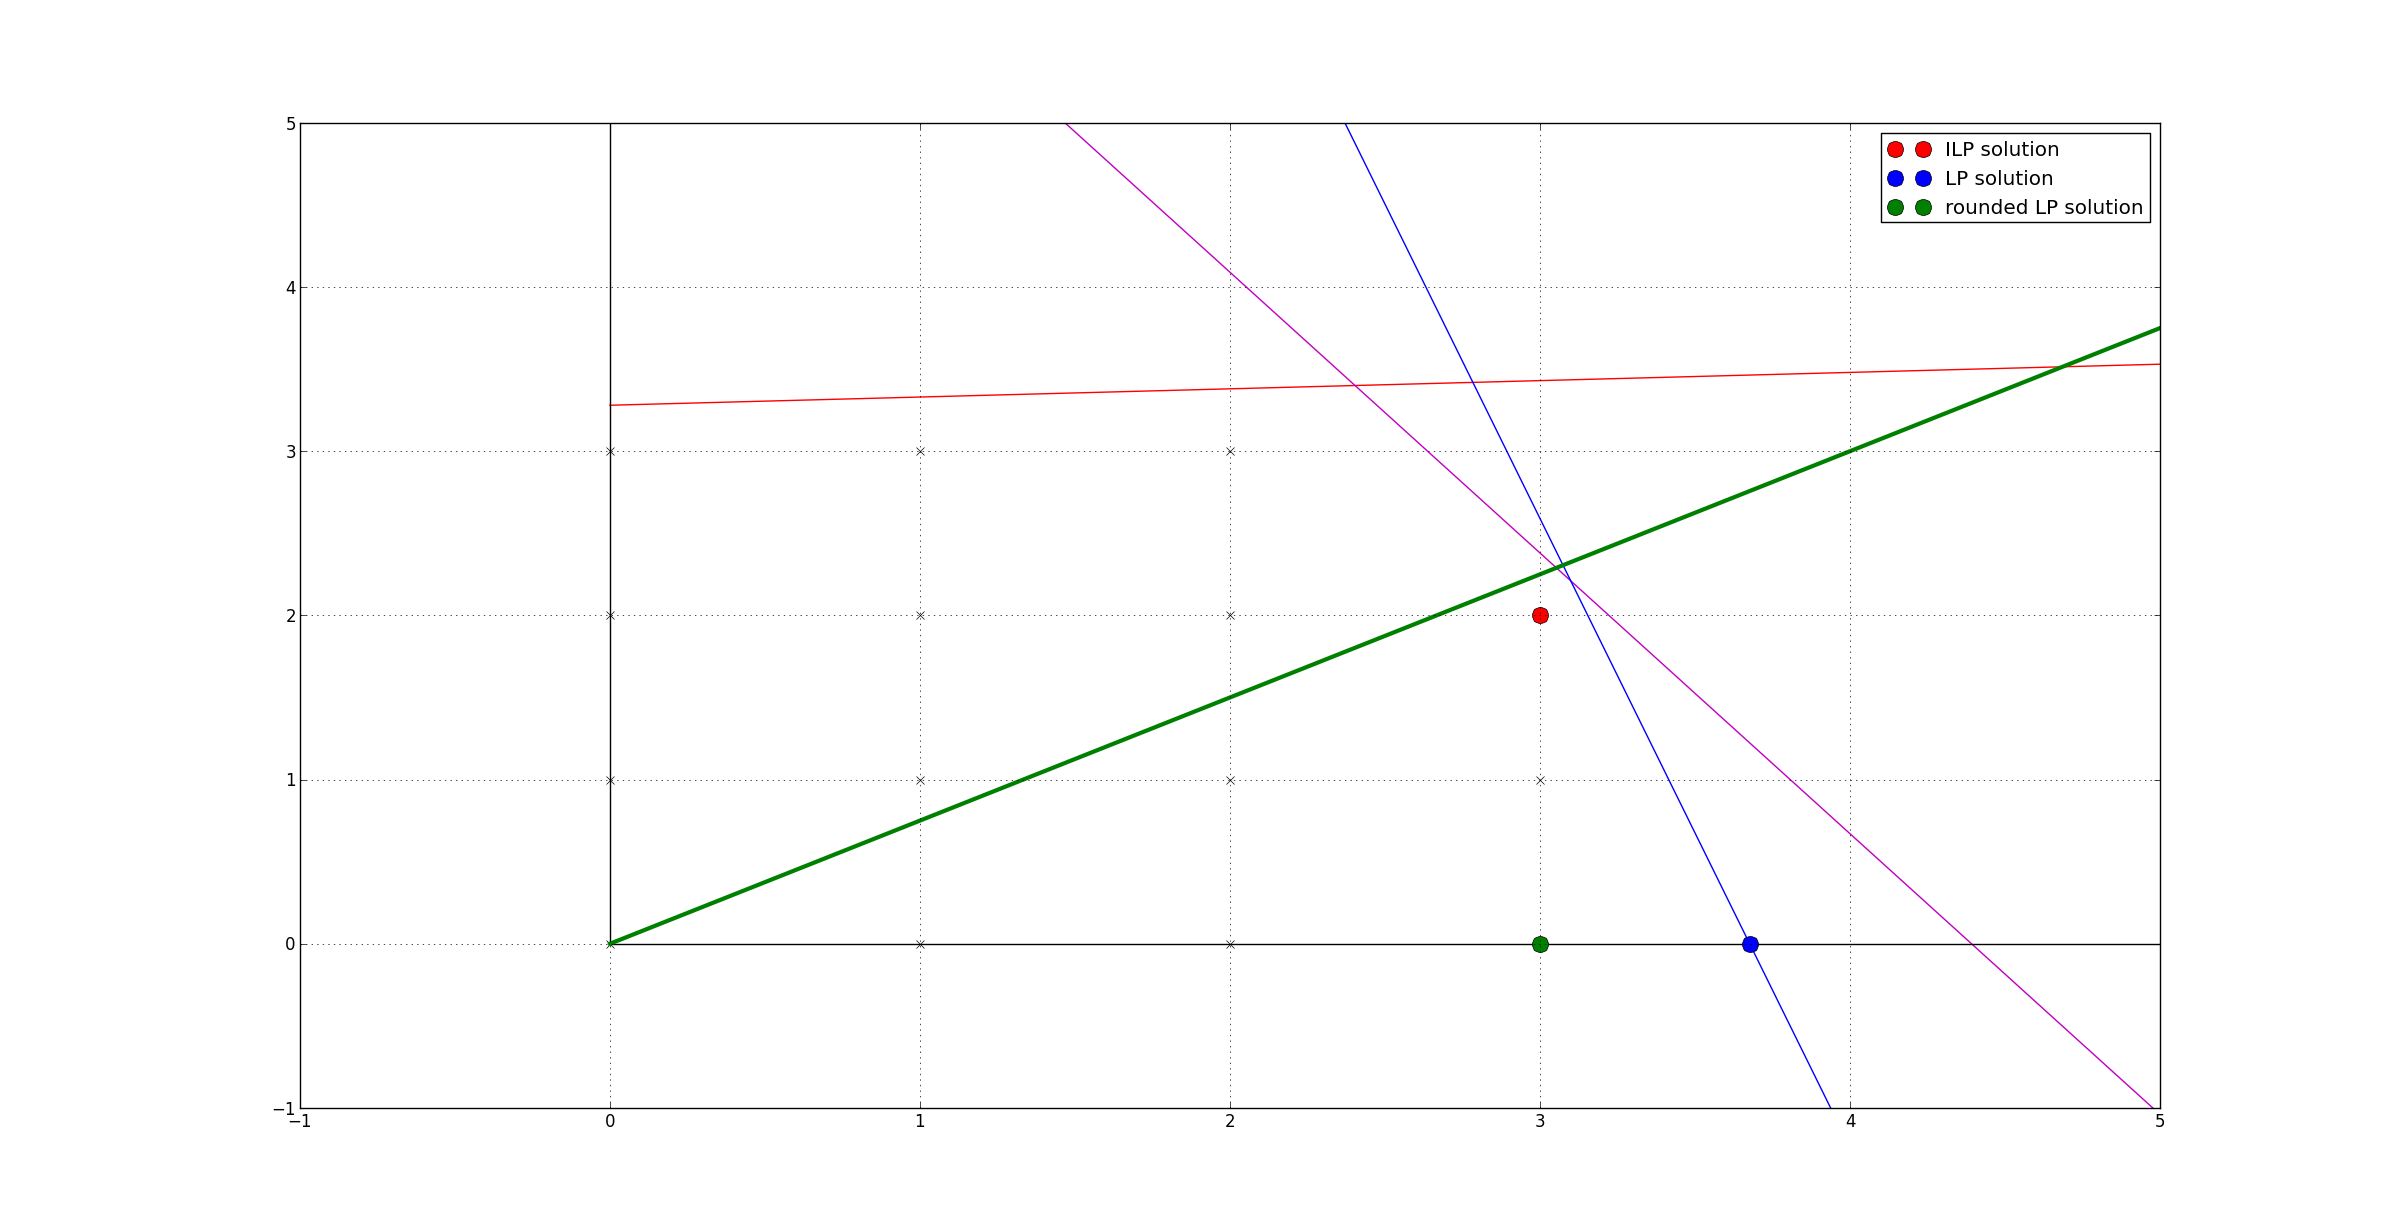
\includegraphics[width=.99\linewidth]{ex3.png}
\caption{BLALABERBLUB}
\end{figure}

\clearpage
\appendix
\lstinputlisting[language=python]{ia_07_01.py}
\newpage
\lstinputlisting[language=python]{ia_07_03.py}
\end{document}